\section{Background}
\subsection{Proving your location}
As an increasing amount of personal information is accessible on the internet and therefore on mobile devices, the security that existed by requiring physical interaction between humans to transfer sensitive data is lost.

\subsection{Ad-hoc networks}

\subsection{Blockchain}

\subsection{Centralised location proof systems}
Location proof systems are expected to be accurate and tamper-proof. For this reason, existing solutions have chosen to use a central authority to issue proofs, or to regulate proof issuance \cite{brassil, luo, khan}.

A hardware technique \cite{brassil} operates by supplementing existing WiFi access points with \textit{femtocells}. A femtocell is a small cellular antenna that connects to a mobile carrier via the Internet. Location verification over the internet is made possible by determining which femtocell a mobile node is connected to as it transfers data via Wi-Fi. This solution requires investment in additional hardware to supplement existing WiFi access points, and requires access to mobile providers' user database to identify users locations.

The use of a centralised system, like that described by Brassil et al. \cite{brassil}, creates security, privacy and vulnerability issues. An attacker who succeeds in compromising the security of the central server can violate the privacy of the users of the system, and potentially track their location. The central system architecture is also vulnerable, in the sense that a resource availability attack such as a DDoS attack could render the central architecture unavailable, making location verification unavailable.

Luo et al. propose a system that uses Wi-Fi access points (\textit{AP's}) to allow users to create location proofs \cite{luo}. In their system, each access point has a \textit{group signature} and can sign location proofs for requesting users. Users can request a location proof from any access point, and receive a proof encrypted by the AP with the group signature, as shown in figure \ref{fig:luo_transaction}. This can then be submitted to a Verifier.

\begin{figure}[H]
\begin{center}
\resizebox {0.6\columnwidth} {!} {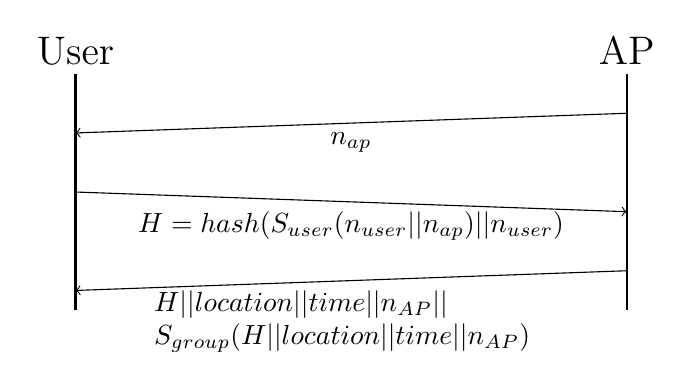
\begin{tikzpicture}
\coordinate (A_T) at (0,3);
\coordinate (A_B) at (0,0);
\coordinate (A_1) at (0,2.25);
\coordinate (A_2) at (0,1.5);
\coordinate (A_3) at (0,0.25);

\coordinate (B_T) at (7,3);
\coordinate (B_B) at (7,0);
\coordinate (B_1) at (7,2.5);
\coordinate (B_2) at (7,1.25);
\coordinate (B_3) at (7,0.5);

\draw[thick] (A_T)--(A_B);
\draw[thick] (B_T)--(B_B);
\draw (A_T) node[above]{\Large User};
\draw (B_T) node[above]{\Large AP};

\draw[->] (B_1) -- (A_1) node[midway,below] {$n_{ap}$};
\draw[->] (A_2) -- (B_2) node[midway,below]
	{$H = hash(S_{user}(n_{user} || n_{ap}) || n_{user})$};
	
\draw[->] (B_3) -- (A_3) node[text width=5cm,midway,below]
	{$H || location || time || n_{AP} ||$\\
	$S_{group}(H || location || time || n_{AP})$};
\end{tikzpicture}}
\end{center}
\caption{Adopted from Luo et al. \cite{luo}}
\label{fig:luo_transaction}
\end{figure}

This kind of system creates \textit{proactive} location proofs. A proactive location proof is one which is created before it is needed. The user creates application-independent location proofs, and can use them at a later time with any application(s) he chooses.